\documentclass[12pt,onecolumn,a4paper]{article}
\usepackage{float}
\usepackage{epsfig,graphicx,subfigure,amsthm,amsmath}
\usepackage{color,xcolor}
\usepackage{xepersian}
\usepackage{graphicx}

\settextfont[Scale=1.2]{BZAR.TTF}
\setlatintextfont[Scale=1]{Times New Roman}


\begin{document}
\title{\lr{ENVISION OF PRODUCT} \\ پلتفرم اینترنتی فروش پوشاک}
\author{امیرمحمد فتاحی\\95000000 \and آرزو دولت آبادی \\000000000 \and امیرحسین ایمانی\\96104087}
\date{\today}
\maketitle

\newpage
\tableofcontents
\newpage
\listoffigures
\newpage


\section{محدودیت محصول}
\subsection{تطبیق پذیری :}

سایت ما باید بتواند با شرایط مختلف تطبیق پذیرد و سازگار شود . برای مثال در صورت عدم موجودی سایت بلافاصله آپدیت شود و عدم موجودی را نمایش دهد . درصورت عدم وجود این موضوع مشتریان نارضایتی از محصول ما خواهند داشت . همچنین سایت باید با تکنولوژی های جدیدی که می آید به روز شود تا سهولت استفاده برای کاربران ایجاد کند .
\subsection{قابلیت اطمینان }
کاربران از ما انتظار دارند که 24 ساعته به آن ها سرویس بدهیم و در سرویس دهیمان وقفه به وجود نیاید . در واقع این ویژگی به انتظار کاربران به استفاده مداوم از پلتفرم ما باز میگردد . کاربران از ما انتظار دارند زمان در دسترس نبودن سایت به دلیل مسائل مختلف و فاصله ی بین این اتفاقات به حداقل خود برسد .

\subsection{مقیاس پذیری }
مقیاس پذیری باید در تکنولوژی ما باشد و بتوانیم با رشد غیر قابل پیش بینی تقاضا به هنگام شویم و غافلگیر نشویم . باید با استفاده از تجهیزات و ساختار ها و زیر بناهای قوی این مقیاس پذیری را در سایت خود ایجاد کنیم .

\subsection{امنیت}
همه ی فرآیند های اینترنتی امروزه به سطوح مشخصی از امنیت احتیاج دارند . یک نوع از امنیت به معنای حفاظت از مشتری می باشد و دیگری به حفاظت از شرکت می باشد . مهندسان سایت ما باید با وقت گذاری تاثیر عدم امنیت در سازمان را متوجه شوند و در صدد حفاظت از آن برآیند .  عمل امنیت باید در دو جبهه صورت گیرد : 1. حفاظت از اینترنت در برابر اسکمر ها 2. حفاظت از شرکت در مقابل دزدان

\subsection{قابلیت استفاده}
در دنیای امروزه قدرت در دست مشتریان قرار دارد . قابلیت استفاده یک محدودیت کالا است که به قدرت مشتری در استفاده از سایت ما باز میگردد . این ویژگی باید شامل
1.	حداکثر زمان بهینه ی پاسخگویی
2.	دسترسی 24 ساعته 7 روز در هفته
3.	قابلیت شخصی سازی نمایش سایت
4.	قابلیت فیلتر کردن اطلاعات
5.	قابلیت انتخاب محصولات
مهم ترین نکته ، در این نکته این است که چند کلیک طول میکشد تا به اطلاعات مورد نظر برسد و یا چرخه ی خود را تکمیل کند .

\subsection{قابلیت نگهداری}
هر چند ماه یکبار قابلیت های جدید به نرم افزار اضافه شود . یک نیازمندی نگهداری باید توسط صاحب سایت مشخص شود و طبق آن پیش رفت .


\section{نیازمندی های کارکردی}
\subsection{ثبت نام مشتری :}
1. ورود به سامانه\\
2. ثبت شماره همراه یا ایمیل \\
3. تکمیل مشخصات\\
4. دریافت پیامک تایید \\
5. تکمیل ثبت نام\\
\\
\\
\subsection{
ثبت نام صاحب فروشگاه  :
}
1. مراجعه حضوری\\
2. تکمیل مشخصات فروشگاه اعم از ساعت کاری و آدرس\\
3. عقد قرارداد با شرکت\\
4. ثبت در سامانه\\
5. دسترسی به سایت \\
6. امکان حذف و ویرایش و اضافه کردن محصولات به همراه مشخصاتشان\\
\\
\\

\subsection{
ثبت نام پیک موتوری  :
}
1. مراجعه حضوری\\
2. ثبت مشخصات خود\\
3. ثبت مشخصات وسیله نقلیه\\
4. ثبت در سامانه\\

\subsection{
ثبت درخواست توسط مشتری :
}
1.	ورود به سامانه\\
2.	دریافت لیست فروشگاه های نزدیک\\
3.	دریافت قیمت پیک\\
4.	انتخاب فروشگاه مد نظر\\
5.	مشاهده کالاهای موجود\\
6.	ایجاد سبد خرید شامل محصولات و تعداد آن ها\\
7.	انتقال به درگاه بانک\\
8.	پرداخت هزینه در سامانه از طریق درگاه بانک\\
9.	مشاهده موفقیت آمیز بودن تراکنش\\
10.	درصورت عدم موفیت تراکنش به گام شماره 7 باز میگردد \\
11.	دریافت محصول\\
12.	ارسال نظر و پیشنهاد به فروشگاه\\
13.	ارسال نظر و فروشگاه به پیک موتوری\\

\subsection{
ثبت درخواست ها توسط پیک :
}
1. تامین تلفن همراه به جهت ردیابی\\
2. قبول سفارش\\
3. دریافت اطلاعات خرید اعم از اطلاعات فروشگاه ، آدرس مقصد و لیست خرید \\
4. تحویل سفارش به مشتری\\

\subsection{
ثبت درخواست مرجوعی توسط مشتری :
}
1.	تماس با تیم پشتیبانی\\
2.	تحویل کالا به پیک\\

\subsection{
ثبت درخواست توسط صاحب فروشگاه :
}
1.	دریافت لیست خرید\\
2.	آماده سازی سبد خرید\\
3.	تحویل سفارش به پیک\\

\subsection{
ثبت درخواست توسط سیستم :
}
1.	نمایش لیست فروشگاه های نزدیک به مشتری و هزینه ارسال پیک\\
2.	بررسی لیست کالا های سفارش مشتری\\
3.	دریافت هزینه توسط درگاه بانک\\
4.	بررسی پیک های موتوری آنلاین\\
5.	انتخاب پیک موتوری\\
6.	نمایش اطلاعات خرید اعم از اطلاعات فروشگاه ، آدرس مقصد و لیست خرید\\
7.	درصورت رد درخواست توسط پیک مجددا جستجو انجام میگیرد\\
8.	دریافت و ذخیره امتیازات و نظرات\\
9.	نمایش امتیازات و نظرات\\

\newpage
\section{برد چشم انداز محصول\cite{3}(\lr{Product Vision Board})}
\begin{figure}[!h]
\centering{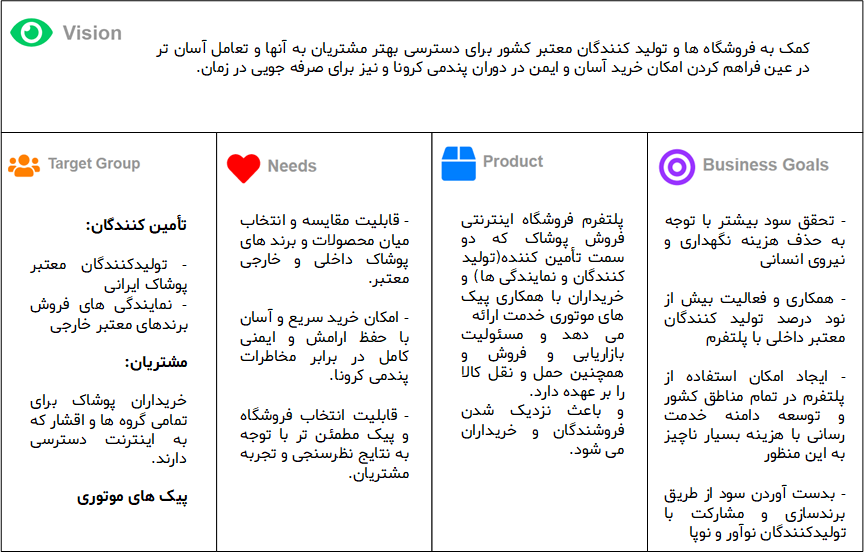
\includegraphics[width=14cm]{product_vision_board}}
\caption{\lr{product vision board}}\label{figpvb}
\end{figure}


\newpage
\begin{thebibliography}{99}
\bibitem{}
فایل توضیح پروژه
\bibitem{}
سایت سجایانگر
\bibitem{3}
\lr{www.romanpichler.com/blog/the-product-vision-board}
\end{thebibliography}




\end{document}
